%!TEX encoding = UTF-8 Unicode

% Load Thesis Class
\documentclass{DEIThesis}

\title{Development of a virtual reality application for the training of cardiac surgeons}

\author{Boscolo Cegion Nicola}
\studentId{2074285}

% Advisor
\advisor{Prof. Savino Sandro}
\graphicspath{ {./res/} }

\university{University of Padua}
\mastername{Computer Engineering}
\academicYear{2023/2024}

\begin{filecontents*}[overwrite]{\jobname.xmpdata}
    \Title{Development of a virtual reality application for the training of cardiac surgeons}
    \Author{Boscolo Cegion Nicola}
    \Language{en-EN}
    \Keywords{Computer Engineering\sep LaTeX}
\end{filecontents*}

% Document

\begin{document}
    % The front matter (Cover, ToC, Abstract, etc...)
    \frontmatter

    % The main content
    \mainmatter
    
    %!TEX root = ../main.tex

\chapter{Introduction}
\label{chp:intro}

\section{Case introduction}

At the university hospital of Padua, 
there is a very important cardiac surgery center where various heart interventions are performed on many people,
the need to teach and visualize the case of operation is very important. \\
Thanks to MRI, surgeons can see not only pictures of the heart, but also can even make 3D models.
Each 3D model can show every detail of the patient's heart, this can make surgeons able to analyze and show where and how to resolve the problem.

\subsection{Virtual reality head mounted displays}

\paragraph{The equipment:}
The equipment: The university of Padua has some Meta quest 2\footnote{All rights to meta reserved} [fig:\ref{fig:metaQuest2}] a \ac{HMD} for \ac{VR}.\\ 
The Meta Quest 2 is a standalone \ac{HMD}, this means that it doesn’t need other peripherals like an external console or \ac{PC} for working.\\
For user interaction, the Meta Quest 2 uses two wireless controllers, but it also has the possibility to use hand-tracking, to let the user navigate the interfaces by using his/her own hands.
The tracking of the user in the real-world environment is achieved using 4 infrared cameras and other sensors like multi axes gyroscopes and accelerometers.\\
They use a custom version of the Android \ac{OS}, this can give a certain degree of liberty in creating APPs for the device.

\begin{figure}[h]
  \centering
  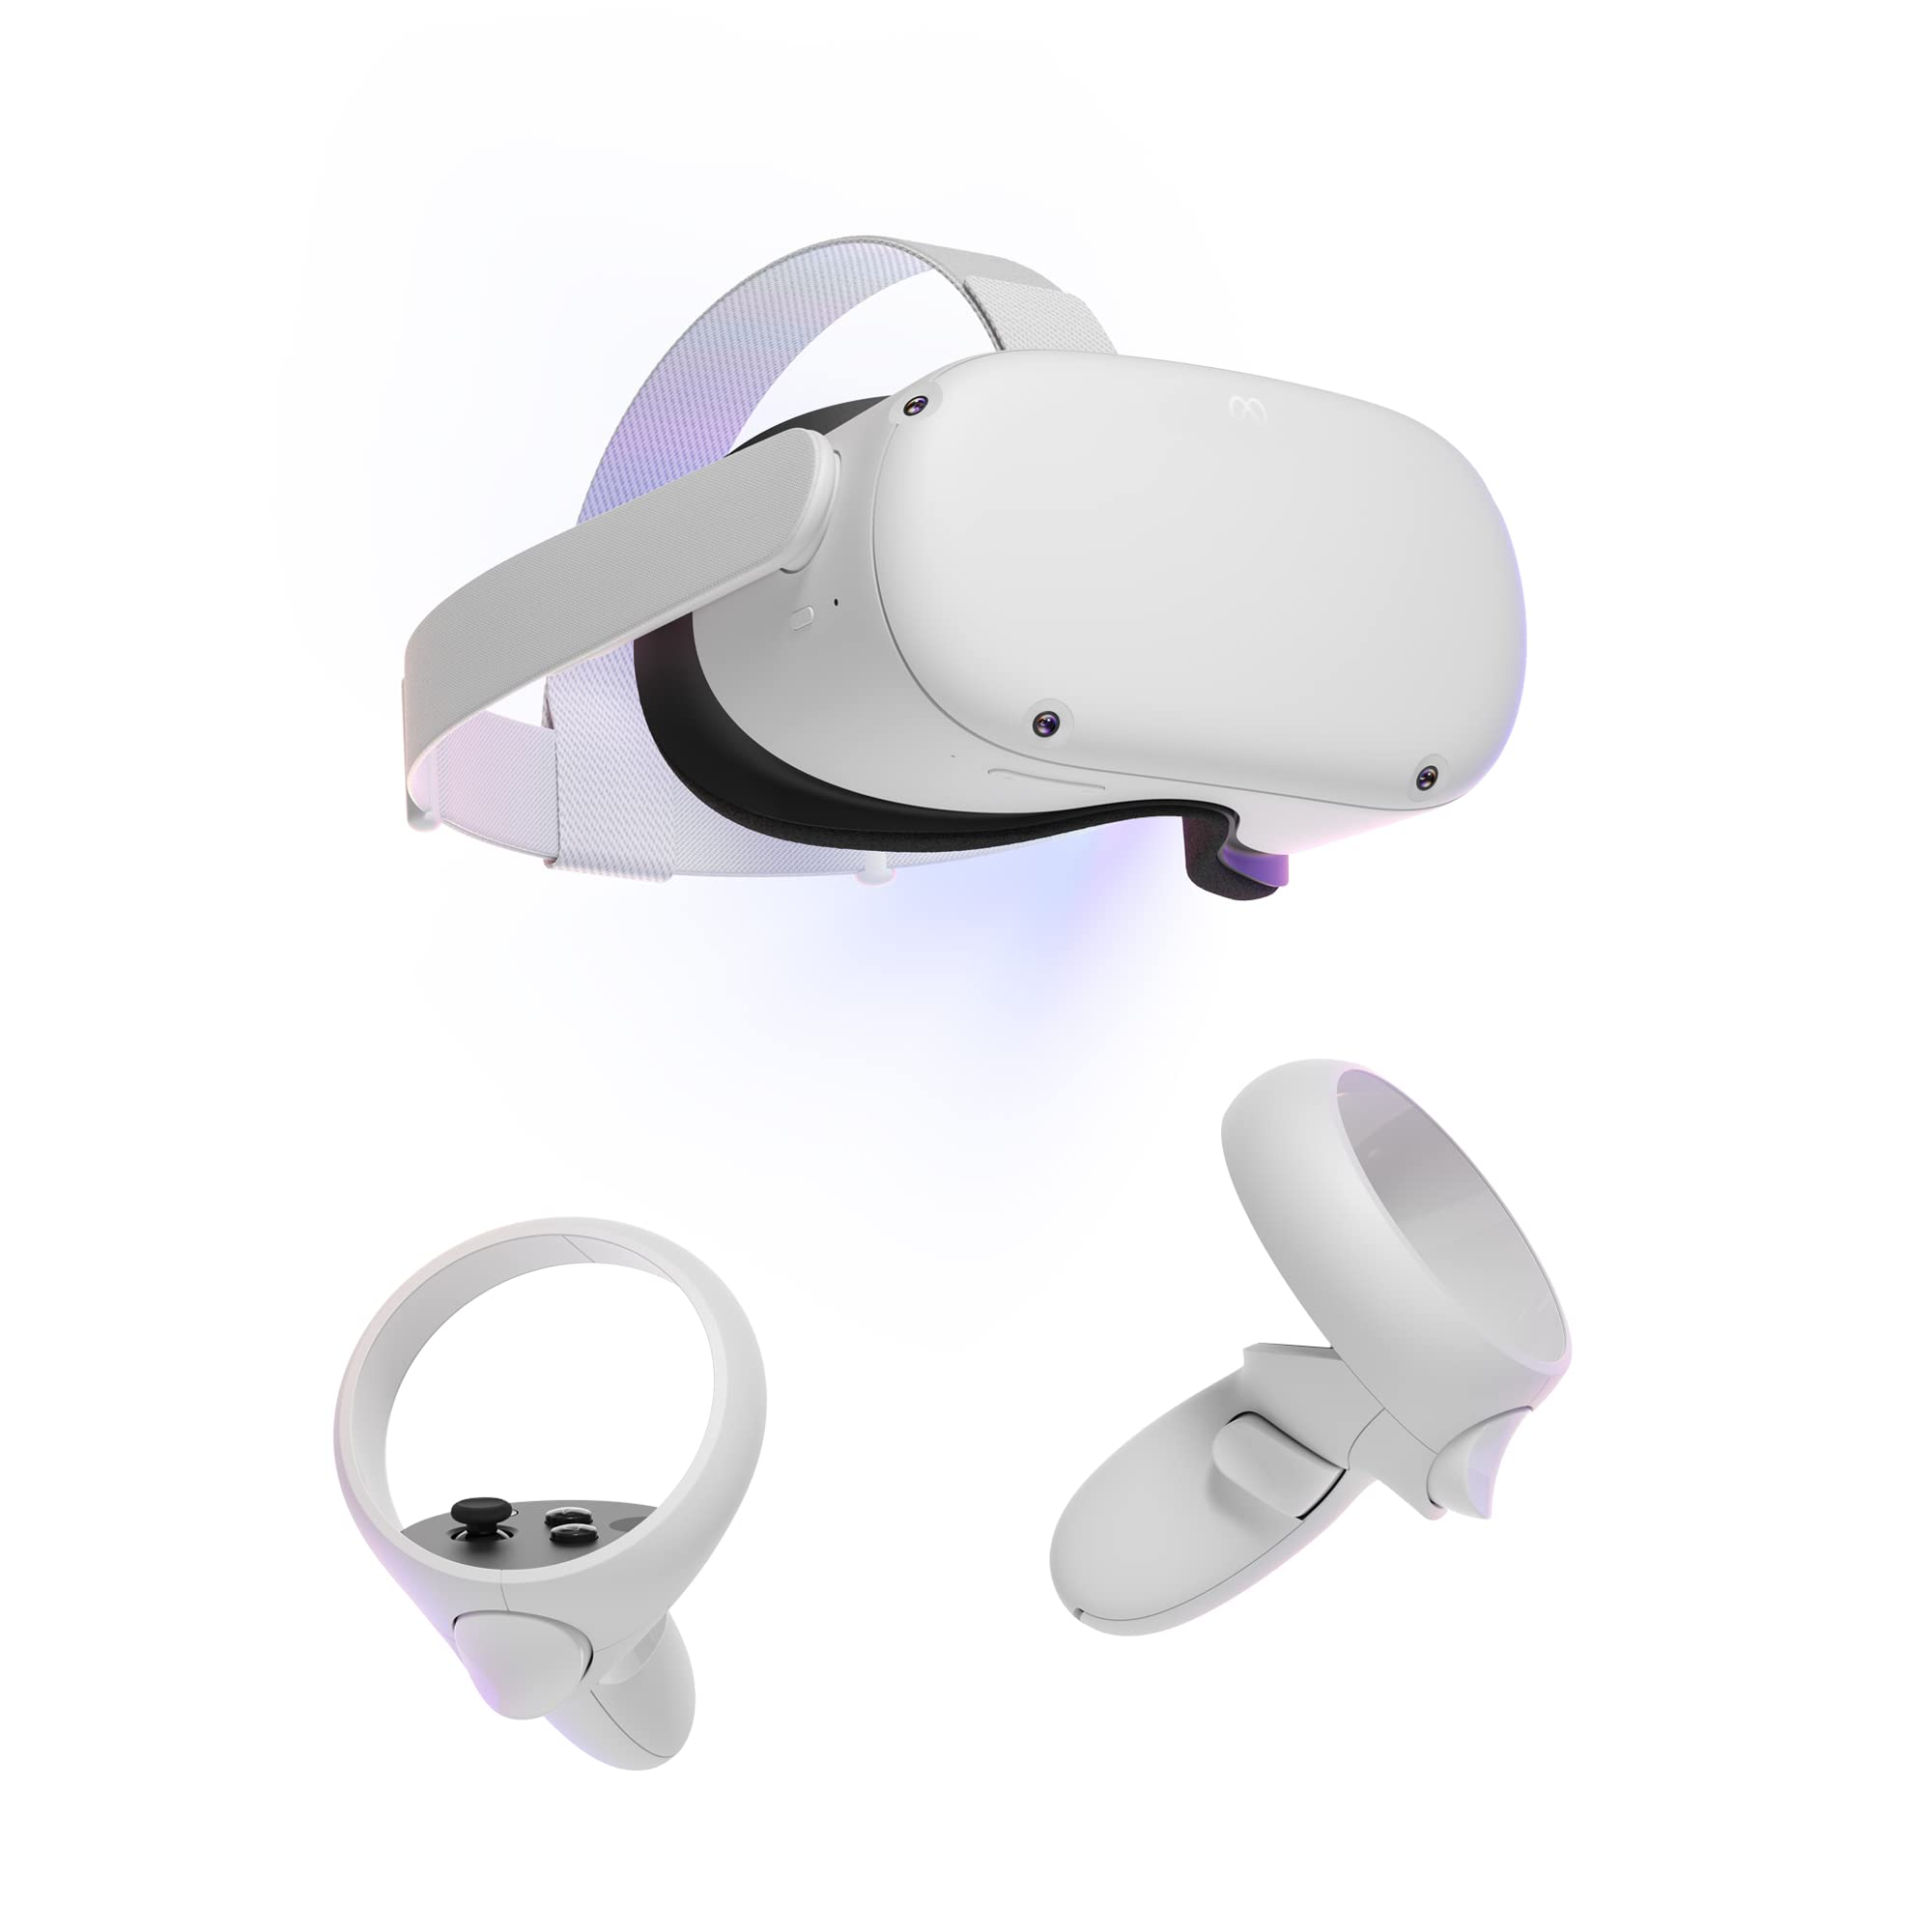
\includegraphics[width=0.5\textwidth]{metaQuest2.jpg}
  \caption{Meta quest 2}
  \label{fig:metaQuest2}
\end{figure}

\paragraph{Use cases of VR:}
Principally the surgeons are using VR equipment for training and showing critical health conditions of different patients' hearts.
They are using an APP called Shapes XR, this APP has a web interface for uploading 3D models and then showing them on the \ac{HMD}.
The app has a multiplayer functionality so that multiple people can look at the 3D models in the environment, even if the developers recommend at max 8 people, they tested with 14 users connected and there weren't any problems.

\subsection{APP problems}

\paragraph{How Shapes XR works:}
Shapes XR lets you create rooms, accessible via a code, where multiple people can create 3D models with basic tools like 3D brushes and standard shapes like cubes, pyramids and so on.
It also lets you upload a 3D model file on their own website, so that in the home you can download it and start to work on it.
It lets you also create your own avatar.
This is the main feature that the surgeons are using for show the 3D Models

\paragraph{The Problems:}
Unfortunately Shapes XR is principally used for 3D modeling, so the app has a lot of features like changing the scale of the world or brushes for modeling the objects that aren't useful for the surgeons,
and quite distracting because for a lot of people it is the first time using a \ac{HMD}.\\
The user experience is extremely important in \ac{VR} because it is difficult to tutoring the user while using the \ac{HMD}.
Then Shapes XR positions the user in an empty 3D plane with little to none point of reference so If a user accidentally uses the teleport function, they may find themselves somewhere far away from the scene they are supposed to be watching.

\paragraph{Feedbacks from surgeons and nurses:}

There was a lesson on 12/12/2023 with the integration of the Quest 2 and Shapes XR. First it was pretty chaotic, a lot of people did not even know how to use the controllers,
 and they had problems even putting in the code for entering the session. Unfortunately we did not have time to make a nice lesson for teaching how to use the HMD,
  the tutorial made by Meta approximates takes 15 min to complete, even more if the user wants to try the mini-games, so we did not have the time to show it. The main critical points were: 

\begin{itemize}
  \item Inadequate tutoring for teaching how to use the \ac{HMD}
  \item Difficulty for accessing the multiplayer room
  \item Difficulty at moving in the room
  \item Some people avatar were blocking the visual of some people
\end{itemize}
\noindent
How we can see a new app for this use case could be useful, and this is the main reason why this project exists. 
    %!TEX root = ../main.tex

\chapter{Requirements}
\label{chp:Requirements}

\section{Functional Requirements}
\noindent
The main features of the project must be:

\begin{itemize}
  \item \textbf{Show custom 3D model at runtime:} The software must be able to download 3D models in OBJ format and render them at runtime, which will also show coloring made by a surgeon. The 3D model should also be movable and have the possibility to change its size. 
  \item \textbf{Multiplayer functionality:} The software must recreate a 3D virtual classroom where a professor can show the 3D model to the students, all students and professor must be synchronized.
  \item \textbf{Upload of 3D models:} There will be a wen app where a surgeon can upload and preview 3D models.
  \item \textbf{Tutoring functionality:} The software will have some tools for learning such as laser pointers, and the possibility to change the position and dimension of the 3D model.
  \item \textbf{Compatibility with Meta quest 2:} The system will need to run on Meta quest 2. 
\end{itemize}
\section{Data requirements}
\noindent
The system necessitates the following data (with the following characteristics) to fulfill its objectives:

\begin{itemize}
  \item \textbf{Required Data:} 
  \begin{itemize}
    \item 3D models in OBJ format.
    \item Local \ac{IP} address for multiplayer.
    \item Generating and managing codes for multiplayer sessions.
  \end{itemize}
  \item \textbf{Data Format:} All data must respect its standard, other communication between clients and server must use \ac{JSON} format file. These formats facilitate data exchange with external systems.
\end{itemize}

\section{Non-functional requirements}
\noindent
To ensure the development of an effective \ac{VR} software, the following non-functional requirements must be considered:

\begin{itemize}
  \item \textbf{Use of Game engine:} A game engine is a software made by another company that is capable of creating a video game, by giving the developers some tools for making the development experience quicker and easier.
  \item \textbf{Simple Back end:} The backend must do the least things effectively because the IT department does not need to update the server that will host the services.
  \item \textbf{Compliance with Internet standards:} The system will be compliant with \ac{HTTP} for all communication between server and client, the \ac{HMD} will use the game engine multiplayer system.
  \item \textbf{Maintaining performance:} \ac{VR} applications need to perform extremely well for having a good \ac{VR} experience, Meta allows a minimum of 72 \ac{FPS}, but our target for a better experience will be 90 \ac{FPS}.
\end{itemize}


    %!TEX root = ../main.tex

\chapter{Preliminary project}
\noindent
The project is made by three main components: \ac{VR} APP, backend, Web \ac{UI}. This chapter will talk about them.
\section{The user experience}
\paragraph{VR APP}
The user experience in the \ac{VR} app will be designed to be intuitive, there will be two types of users: professors and students.
Professors will have the ability to create a virtual classroom. Students can join these rooms by entering a unique code provided to them. Once inside, the professor will guide the lecture by showcasing 3D models of different hearts.
They can manipulate these models by moving, resizing, and using a laser pointer to highlight specific areas of interest. 
\paragraph{WEB UI}
The Web app will let the professor to upload any OBJ models needed for the lecture by a simple form, and the web app will allow to view 3D models.

\section{The VR APP}
\noindent
This section will explain the main choices behind the \ac{VR} APP
\paragraph{The development environment:} 
There are three main way to develop on the Meta Quest 2:

\begin{itemize}
  \item \textbf{Native:} By using native \ac{API} that Meta provides for the \ac{HMD}.
  \item \textbf{Unity:} Is a famous game engine principally used for lightweight video games, It is pretty functional and easy to use, its programming language is \texttt{C\#}. 
  \item \textbf{Unreal Engine:} Is a famous game engine used for big games, its performance is the best in the market, it uses \texttt{C++} and a graphical programming language called Blueprint.
\end{itemize}
\noindent
As we said in the non-functional requirements we will use a game engine, I have opted for \ac{UE} because of its performance, the 3D models that will use are complex (\textasciitilde1-10MBytes in size),
so it will be used for its performance, also it has a lot of tools for multiplayer and a good documentation other than a big community of developers.

\section{Unreal Engine}
\noindent
Made by Epic Games, the project was born for the video game Unreal,
now it is one of the best engines that power a lot of important video games and 3D animation. 
For this project it will use the 5.2.1 version because at the time of writing this thesis for the best compatibility with the \ac{HMD}. 
The main reason for this upgrade was for faster building time and more advanced \ac{API} of Meta. 

\paragraph{The fundamentals:}
\ac{UE} has a 3D preview mode that lets the user set the various 3D objects in the scene.
In unreal a scene is called "Level", each element in a level is called "Actor", Actors are made by multiple components.\\
Each element of unreal can be built with a proprietary system called Blueprint, a visual programming interface, or via \texttt{C++}, or by combining them.
Principally Blueprint can make the development of the project faster and easier at the cost of performance, \texttt{C++} performs better, and it has a bigger range of tools.
So It is important to combine both languages for having the best performance and flexibility in the project.\\
Like a lot of game engines, \ac{UE} tries to render many frames as much as possible, each cycle of rendering is called tick.\\
It's important that long actions must be asynchronous with respect to the game ticks, and if something must be a runner in the so-called "game thread", it must be as fast as possible so that the frame rate does not drop to a certain level.\\
Another important component is the player controller, this is the instance of a player inside a level, a player controller can possess a pawn actor or a character actor.


\paragraph{External library:}
One challenge for this application is having a correctly multiplayer session between \ac{HMD}, unfortunately \ac{UE} does not provide a \texttt{VRpawn} that has multiplayer functionality.
For having a faster developing experience, a library called VRexpansion\footnote{\url{https://vreue4.com/}} will help the development, the library is open source under MIT licensing.
The main useful components are:
\begin{itemize}
  \item \textbf{VRcharacter:} a character for \ac{VR} games, all its components can be replicated in a multiplayer session.
  \item \textbf{Grippable Interface:}  interface that can enable actors or static meshes to be gripped by the \ac{HMD} components. It also can be replicated in a multiplayer session.
\end{itemize}

\paragraph{Events:}
Events are what start the execution of code inside a Blueprint. Each blueprint have its own standard event, they depend on the object, the basic ones are:
\begin{itemize}
  \item \textbf{Begin Play:} runs one time when the actor is spawned (this is not a constructor).
  \item \textbf{On tick:} runs on every game tick.
\end{itemize}
\noindent
We can also create custom events with Blueprint or \texttt{C++}, they can be triggered whenever we want, they can also be replicated in clients in multiplayer sessions. 
Like functions, events can have inputs but not outputs.

\paragraph{Multiplayer:}
\ac{UE} just supports a client-server configuration for managing multiplayer sessions, it has two main implementations: Stand-Alone server and listening server.\\
A Stand-Alone server consists in having a server that emulates the gaming session, it requires a server powerful enough to run the basic function of the game event if it does not need to render it.\\
A Listening Server does not need a Stand-Alone server, simply one device acts not only as a client but also as a server. Normally client-server is the best in performance and latency, but because this software is simple, the listening server is the right implementation.\\
For making a good multiplayer we have some blueprints that can help with the synchronization of the data: 

\begin{itemize}
  \item \textbf{Game Mode:} runned only inside the server, as it is called it provides the rules how the game should work, it is important for the login and log out of the players.
  \item \textbf{Game state:} it represents the state of the game, all \ac{HMD} has one, but it is always replicated by the server.
  \item \textbf{Player controller:} runned in every \ac{HMD}, it represents the player using the \ac{HMD}.
  \item \textbf{Player state:} it has all the data of a player like the username, its replicated.
\end{itemize}
\noindent
An important feature for synchronize events between client and server are \ac{RPCs}, \ac{RPCs} are events of actors that can per reproduce in multiple device at once by following one of these rules:
\begin{itemize}
  \item \textbf{Client:} The \ac{RPCs} are executed on the owning client connection for this actor.
  \item \textbf{Server:} The \ac{RPCs} are executed on the server, it must be called from the client that owns this actor.
  \item \textbf{Multicast:} The \ac{RPCs} are executed on the server and all currently connected clients the actor is relevant for, Multicast \ac{RPCs} are designed to be called from the server, but can be called from clients. A Multicast \ac{RPCs} called from a client only executes locally.
\end{itemize}

\paragraph{Multiplayer}
Since multiplayer is one of the fundamentals of modern gaming, \ac{UE} provides a suite of tools to help achieve it.
Unfortunately, some of these tools will be unusable because, at this time, we cannot publish the app to the Meta Quest store.
This limitation will restrict the multiplayer capabilities, allowing us to create only a LAN-based multiplayer mode, meaning that the \ac{HMD}s must be connected to the same local network.

\section{Network Infrastructure}
\noindent
The Network Infrastructure [fig:\ref{fig:NetworkSchema}] it is simple, a server will be hosted in the IT department of the hospital that will host the \ac{REST} server for managing 3D Models and multiplayer sessions,
and in the same server will host via NodeJS the Web Portal for managing the 3DModels.
The multiplayer itself will be manage by the host \ac{HMD}

\begin{figure}[h]
  \centering
  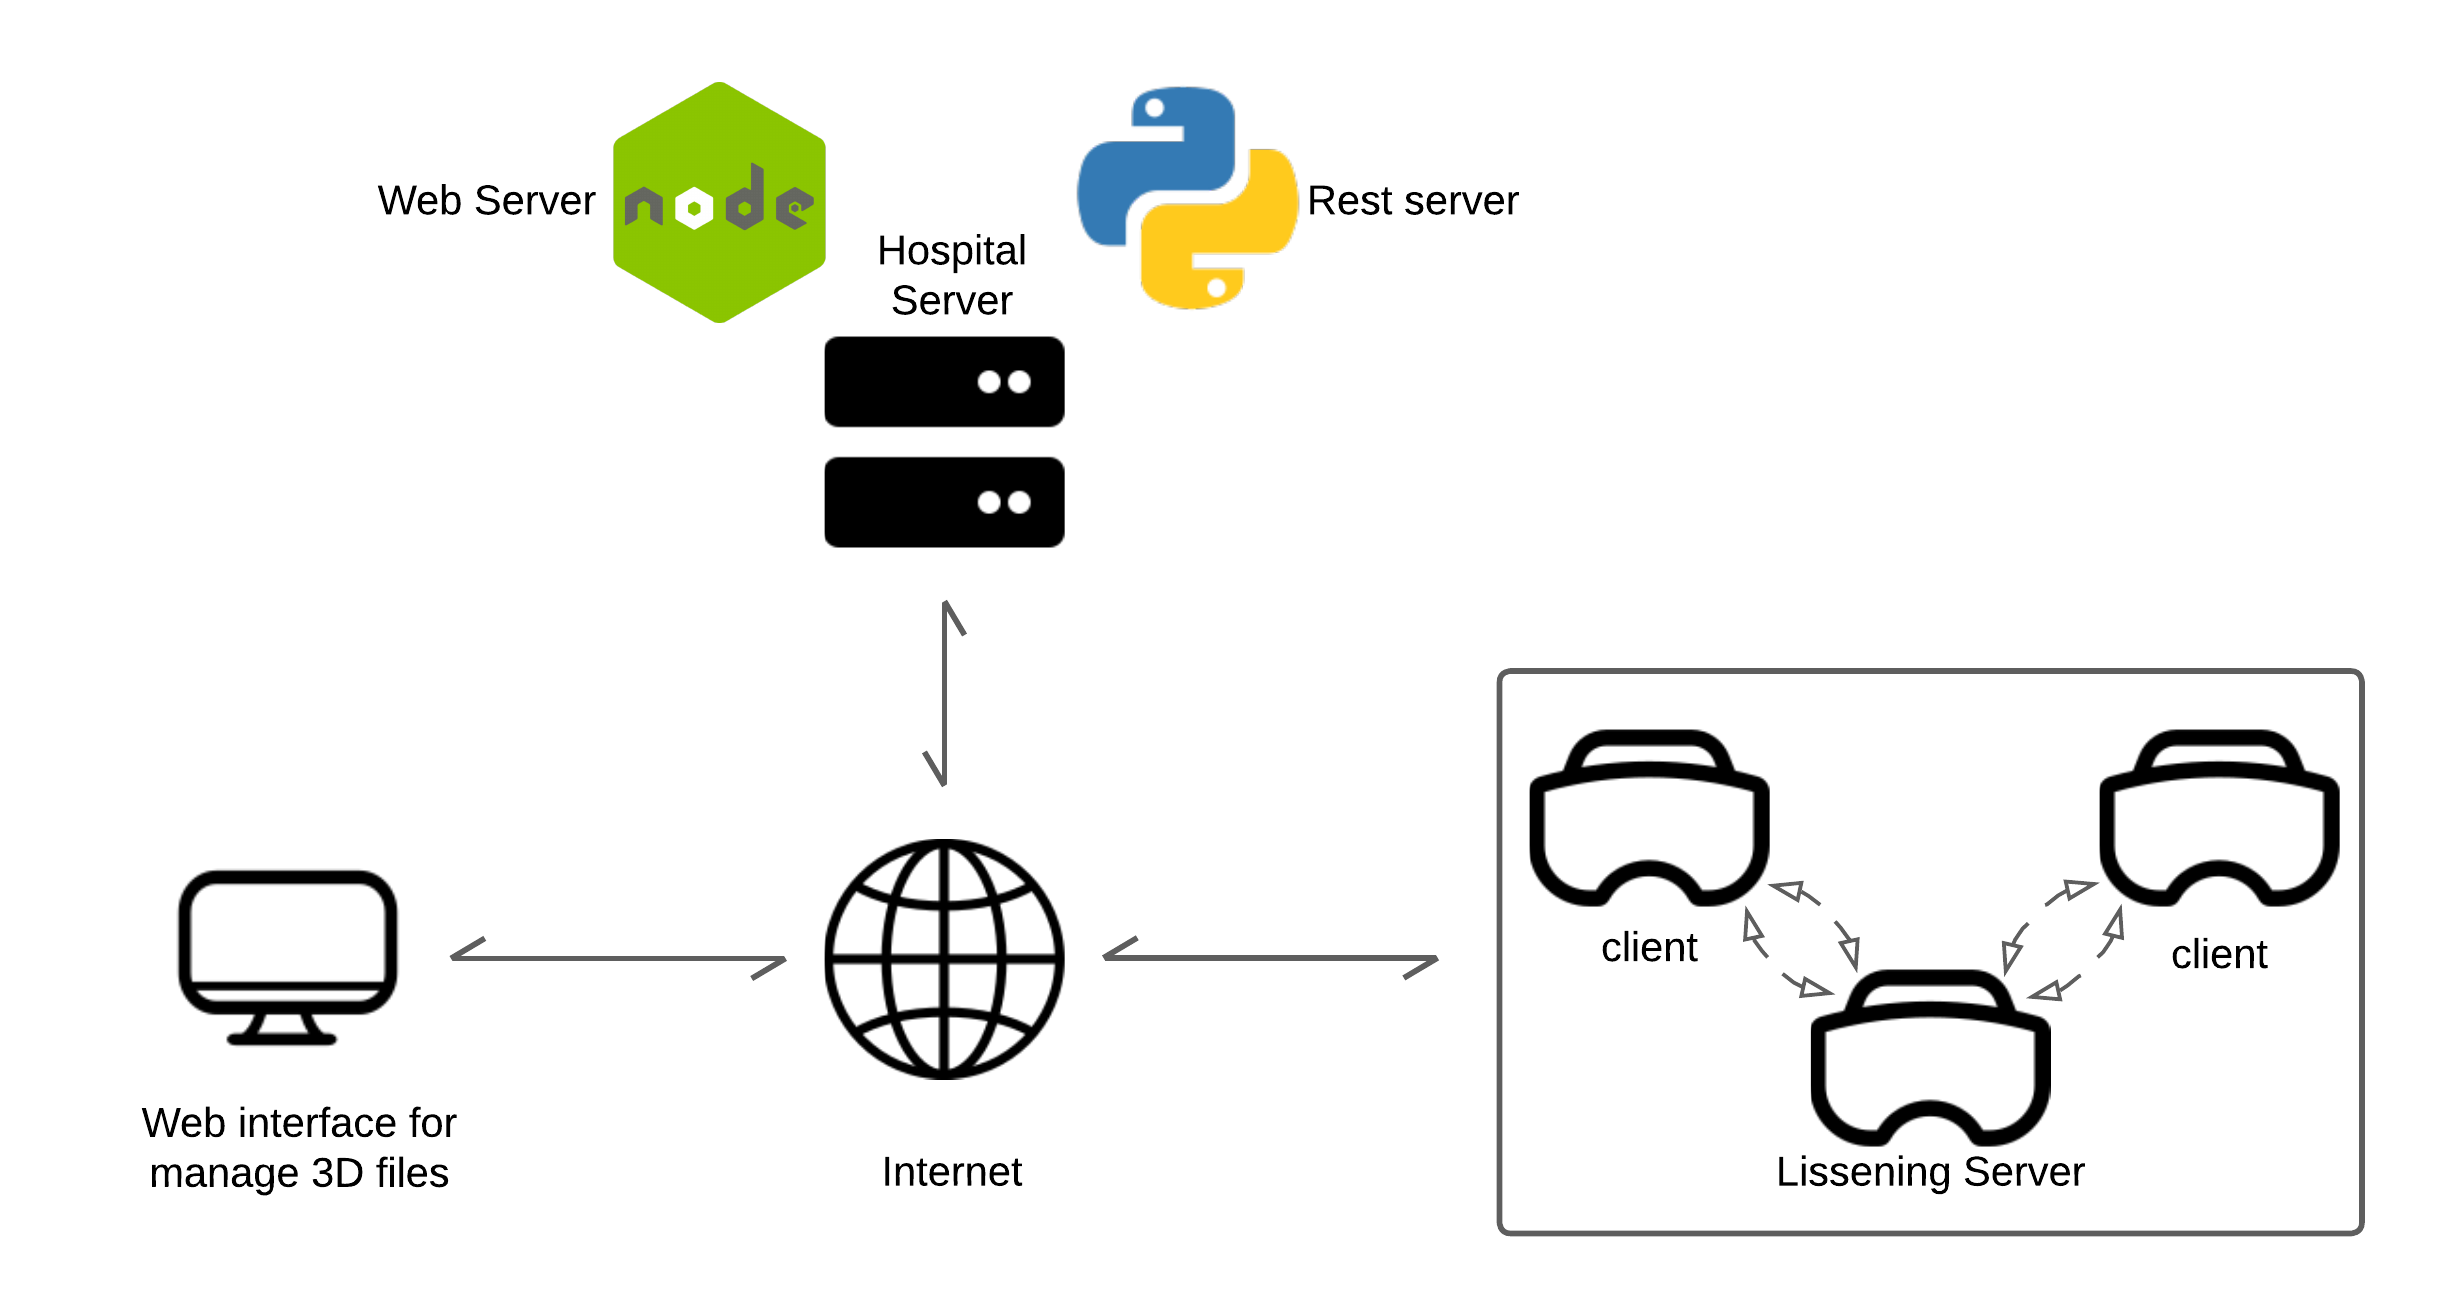
\includegraphics[width=\textwidth]{networkSchema.png}
  \caption{Network Schema}
  \label{fig:NetworkSchema}
\end{figure}


\paragraph{The backend:}
The backend is a simple Python program that functions as a \ac{REST} server, where each 3D model is a resource.
It also manages the multiplayer session by creating the session code, and saves the \ac{IP} address of the listening server.
The library used is called Flask\footnote{\url{https://flask.palletsprojects.com/en/3.0.x/}}, it simply lets you run a function with respect to a \ac{HTTP} response received.

\paragraph{The Web UI:}
The Web \ac{UI} is made with ReactJS, a popular framework for website, the main reason of this choice is for faster development because its community is massive, in fact will be using a UI library called MUI\footnote{\url{https://mui.com/}}
and a 3D library for rendering 3D models called React Three Fiber\footnote{\url{https://r3f.docs.pmnd.rs/getting-started/introduction}}.\\
The main functionality of the Web \ac{UI} will be:
\begin{itemize}
  \item previewing 3D models with the right colors 
  \item upload 3D models
  \item delete 3D models
\end{itemize}


\section{Development environment}
\noindent
It is important to set the right development environment for this project, even if for the Web \ac{UI} and backend it is a standard NodeJS and Python environment, 
it is not that simple for \ac{UE}\\
First the choosing the right version is very important because Meta does not always test all \ac{UE} version, at the start of the developing of the project, the last one was 5.2.1,
we also need Visual Studio with the right components for compile in \texttt{C++}, we could use other text editor, but Visual Studio is the most completed one for unreal.
For other information look at: \cite{UEvisualStudio}
After we set up the basic \ac{UE} environment, we have to pick the right Android studio and \ac{SDK} for building for Android \\
Another important component is the Android \ac{NDK} that enables \ac{UE} to compile native \texttt{C++} code.
But for installing there is a command line tool that \ac{UE} shipped with that can install the right version. 
Because the requirements differ with respect to the version of \ac{UE} for more information look at Epic Games documentation: \cite{UEandroid}.\\
Other than the configuration for Android, we also need to add the right components for building for the Meta Quest 2,
There are two other components useful for developing:
\begin{itemize}
  \item \textbf{MetaXRPlugin:} plugin for: sideload, publish and setting the project for the \ac{HMD}, this component is already implemented in the \ac{UE} fork of META.
  \item \textbf{MetaXRSimulator:} simulator for the \ac{HMD}, this is extremely important because the compile time of the \ac{APK} is slow. The simulator uses a PC instance of the game, and it overlays it.
\end{itemize}
\noindent
For more information look at: \cite{MetaSetup}


    %!TEX root = ../main.tex

\chapter{The project}
\label{chp:project}
\noindent
This chapter will explain the development behind the project by starting from the fundamentals.
\section{The 3D models}
\noindent
In this section will talk about how 3D models are saved and rendered on \ac{UE}
\subsection{The OBJ file format}
\noindent
For understanding how \ac{UE} will show 3D models and how they will be stored, we must talk about their characteristics.

\begin{itemize}
    \item \textbf{Vertices:} points that describe the geometry
    \item \textbf{Faces} indicated were there is a polygon by grouping 3 or more vertices 
    \item \textbf{Normal:} there is one for each vertex that is in a face, indicates the direction to which the face is exposed, and for calculating how light is reflected
    \item \textbf{UV:} vectors that helps how a texture should be applied to the model
    \item \textbf{Vertex colors:} RGB vector that indicates a color for each vertex
\end{itemize}
\noindent
As we talked about in chapter \ref{chp:Requirements}, we will use the OBJ file format for storing files.
The React Three Fiber has a native support for OBJ, and the backend server does not need to read the file but just to manage by saving, deleting and sending it via \ac{HTTP}.
Unfortunately \ac{UE} does not have a OBJ file reader usable at runtime but just an importer for what it calls static meshes (3D models that don't have moving parts).
So there is the need to build a parser OBJ to \ac{UE} custom types.\\
First we need to understand how the OBJ file format is compose of, here a general example code:\ref{code:OBJExample}

\lstinputlisting[float=h, language=Octave, caption=OBJ file example,style=obj, label={code:OBJExample}]{code/exampleOBJ.txt}
\noindent
The vertices, UV and normals are simply written, instead the faces have different formats, first not always they use triangles, but also quads, this depends on how the file was exported.
For ease of use the parser will support both. The numbers of the face are the indices of the vertex. Indices start from 1.
A face can also have the UV and normals corresponding for the vertex. For our use cases UV aren't needed, but for future-proof they are still being parsed correctly.\\
Sometimes it is useful to divide the 3D model into multiple objects the OBJ format represents by dividing the 3D model with a "\texttt{o}".
OBJ can also divide the faces in groups by dividing them with a "\texttt{g}".
Here an example of how the division works: code:\ref{code:OBJgrouping}

\lstinputlisting[float=h, language=Octave, caption=OBJ grouping,style=obj, label={code:OBJgrouping}]{code/exampleOBJGrups.txt}
\noindent
The software that the surgeons are using for exporting 3D models just support groups, so will implement those, and they will become useful for rendering the model in parts.

\subsection{To unreal types}
\noindent
\ac{UE} has some custom classes formanaging things like vectors, colors... These classes also to have useful methods that also interface with the blueprint system, we can for example expose variables or functions, so we can call them at blueprint level.
This is very important so that we can interconnect the \cpp components with blueprints.\\
Unreal has a component called \texttt{procedural mesh}, this component has the possibility to render a 3D model given vertices and triangles, it also has more data that you can feed to the rendered mesh such  us: normals, tangents, UV, vertex colors.
It can also have collisions and a material.\\
The \texttt{procedural mesh} also has the possibility to load the mesh in parts, so the parser will save the different triangles in the various groups that are defined in the file.
This will be important later for loading time.\\
Vertices are directly read and saved in an array of \texttt{FVector} and normals will be saved in the same way.
Vertex colors just need to be read and put in a \texttt{LinearColor} array, the object itself can be initialized with the data retrieved in the file.
UV because are 2D vectors will be saved in an array of \texttt{Vector2D}.
Unfortunately there is a mismatch between how \ac{UE} manages correlation between vertices and normals respect the OBJ file standard.
Unreal needs two arrays that contain vertices and normals, so that the vertex in the array at the position \texttt{i} must have its normal in the normal array at position \texttt{i}. 
This is still a trivial problem, because there's just the need to load all the normals in memory and then save them again in the correct order decided by the faces.\\
UVs are being managed in the same way.
Another problem is that unreal just accepts triangles and not quads, and because it is a common practice to use quads when exporting 3D models the program will convert quads in triangles, this is pretty trivial, for each quad we can divide it in two triangles.\\
Unreal also works in \texttt{Z}-up coordinates that means that the \texttt{Z} axis points up, there is another standard called \texttt{Y}-up were the \texttt{Y} axis points up, unfortunately the OBJ file format does not have any ways to reference scale or if the file is saved in \texttt{Z}-up or \texttt{Y}-up,
so it is important to export the file in \texttt{Z}-up.\\

\begin{figure}[h]
    \centering
    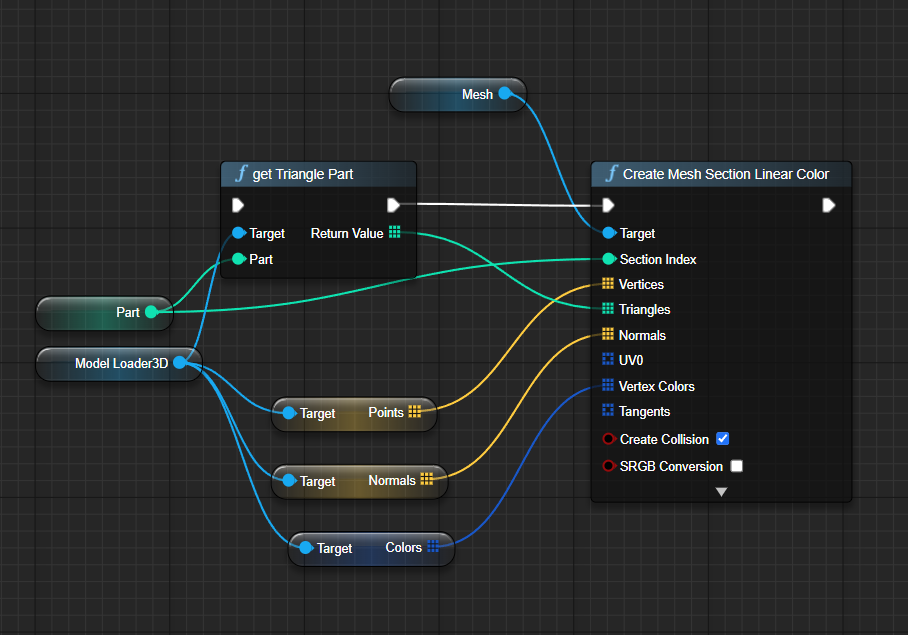
\includegraphics[width=\textwidth]{blueprints/loadingMesh.png}
    \caption{Add mesh section blueprint node}
    \label{fig:loadingMesh}
\end{figure}
\noindent
Because when loading a big procedural mesh it could create a big loss in \ac{FPS}, for reduce this problem the model will be rendered in parts, by using the different groups found on the file. After some testing I have decided to load groups every \texttt{0.6ms}. 

\section{The user interface}
\noindent
Thanks to the VRExpansion plugin, we can use the standard \texttt{VRCharater}, this \texttt{Character} has already implemented the online synchronization, and it also has the components for the controllers and camera management.
The controllers can \texttt{grip} any \texttt{Actor} or \texttt{Component} that implements the interface \texttt{VRGrip}, this will be used for  moving the 3D models.
Other than that the \texttt{VRCharater} is an empty blank, and will need to implement some functions for making it fully functional.\\
Here are the main components to develop:

\begin{itemize}
    \item Input management
    \item Widget Interaction
    \item Interaction pointer
    \item Side menu
    \item Grip framework
    \item 3D model size management    
    \item Loading sphere
\end{itemize}

\subsection{Input management}
\noindent
Input in \ac{UE} is managed by two data files: \texttt{Input Action }and\texttt{Input Mapping Context}.
In the next two paragraphs will be addressed how the input works, and then will be used in the various components of \texttt{VRCharater}.

\paragraph{Input Action}
Are files that are used to identify a certain input of the controller, each file should be named after an action more than the input used for making clear what they serve.
For example:\\
For using the \texttt{A} button find find in the right controller,
you need to have a file that represents the button,
the necessary settings are: Consume input which allows you to take into account that the input has been served,
and the type of value that in this case will be \texttt{Digital (bool)}.

\begin{figure}[h]
    \centering
    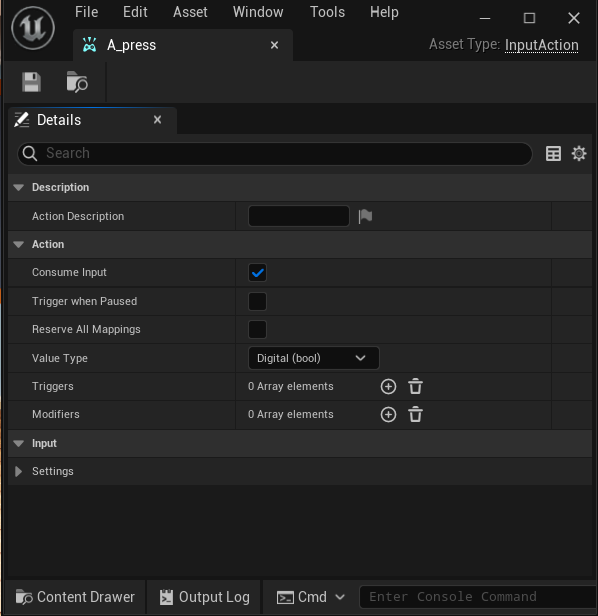
\includegraphics[width=0.7\textwidth]{blueprints/InputActionExample.png}
    \caption{Input Action example}
    \label{fig:InputAction}
\end{figure}

\paragraph{Input Mapping Context}
Files represent all the inputs used by an actor, an actor could change its inputs, so they can be multiple files for different occasions,
Here each \texttt{Input Action} will be associated with the corresponding input.
\texttt{Input Mapping Context} can be used for other objects so that they can override the standard behavior of the \texttt{Character}, for example by equipping a laser pointer and using the \texttt{A} button for toggle it.
Each \texttt{Input Mapping Context} can be bound with different controllers, this can be useful if we will be porting the app for another \ac{HMD}.
For setting the \texttt{Input Mapping Context} there is a function called \texttt{Add Mapping Context}.

\subsection{3DmodelVewer actor}
\noindent
The \texttt{3DModelActor} is a custom actor designed to facilitate the visualization of 3D heart models that is an extension of \texttt{Grippable Actor}. This actor comprises four primary components. The first component is the Procedural Mesh, which utilizes Unreal Engine's capabilities to generate and display a heart model in real-time. 
The second component is a Loading Indicator \texttt{Sphere} that provides visual feedback during model loading processes informing users about the ongoing operations. In addition, the \texttt{3DModelActor} features a \texttt{Text Component} that displays error messages when issues arise during the loading of the 3D models.\\
The core functionality of the actor is driven by a custom \texttt{Model Loader}, This custom component is responsible for fetching 3D models from online sources, parsing the model data, and integrating it into the procedural mesh and it implements the OBJ parser.\\
The \texttt{Model Loader component} can download the 3D Model from the backend thanks to the function httpFileDownload, that thanks to a delegate, can be runned in an asynchronous way thanks to \ac{UE} threads, and then notify when the execution is complete.
Another functionality of \texttt{3DModelActor} is that it can be gripped thanks to its parent Blueprint \texttt{Grippable Actor}.

\lstinputlisting[language=C++, caption=model loader header file, label={code:model loader}, linerange={12-74}, style=cpp]{code/c++/model loader.h}

\subsection{Widget Interaction}
\noindent 
In a normal application we are used to managing input mainly via mouse or touch screens, in \ac{VR} we can not have that, so It's important to create some kind of \ac{UI}.
One of the most used approaches is showing some kind of virtual display with buttons so that the user can interact, for this will be using a blueprint called \texttt{Widget} and will be explained in here ""INSERT CHAPTER"".
Unfortunately \texttt{Widgets} are used for 2D menus but thanks to an actor component we can use it in a 3D environment.\\
For interacting with a \texttt{widget} in a 3D space, \ac{UE} has a component called \texttt{widget interaction} that can evaluate if it is pointing to a \texttt{widget}, it can also give the world location of where it is pointing. This component will be attached to each \texttt{grip motion controller component}.
For letting the user see exactly where the controller is pointed, when the controller is near the \texttt{Widget} a trace will be shown.
For the trace will be used a Component called \texttt{Spline Mesh}, as the name suggests, uses various points and interpolates a mesh for creating a complex curve.
Still our use will be simply by just using two points Fig[\ref{fig:splineExample}]. So the algorithm is simple: each tick a function called \texttt{InteractionPointer} will control both controllers if the \texttt{widget interaction} points to a \texttt{Widget}, then will draw the spline.



\begin{figure}[h]
    \centering
    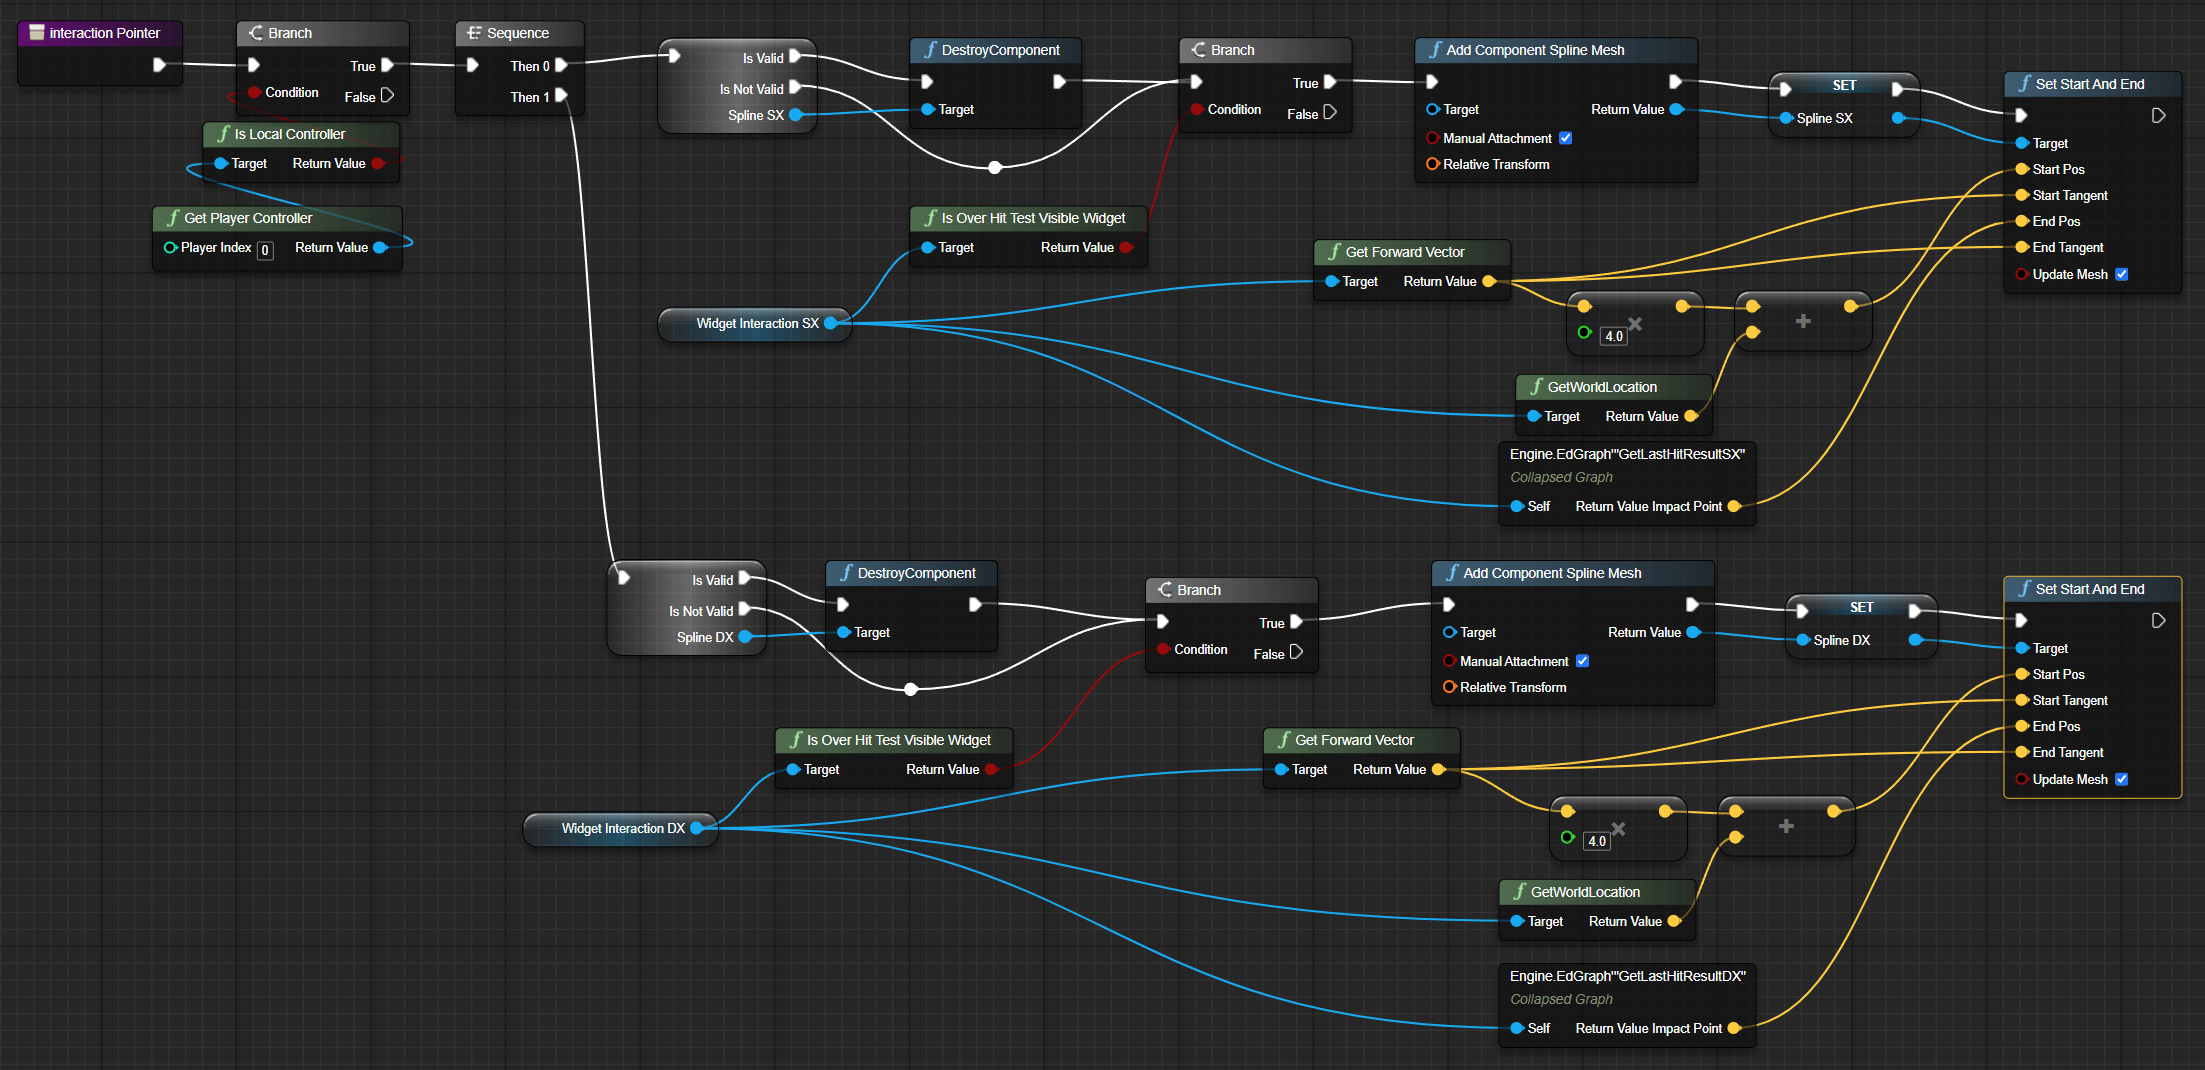
\includegraphics[width=\textwidth]{blueprints/interactionPointer.png}
    \caption{Widget Interaction code}
    \label{fig:InteractionPointer}
\end{figure}

\begin{figure}[h]
    \centering
    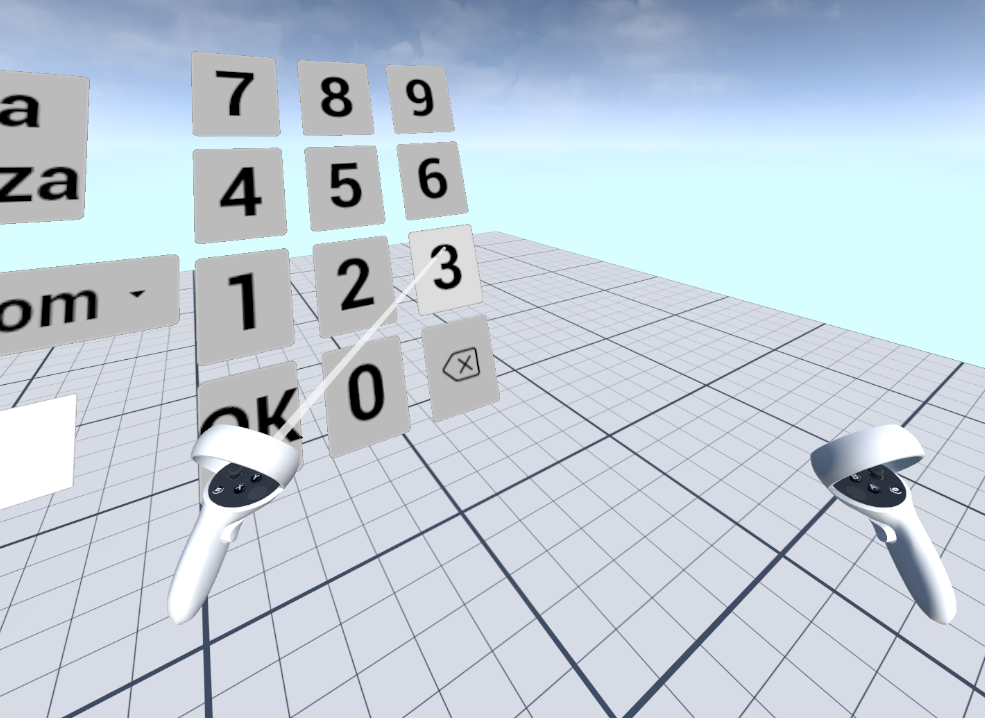
\includegraphics[width=0.8\textwidth]{vrScreenshot/splineExample.png}
    \caption{On the left a controller that create the spline pointing to the widget}
    \label{fig:splineExample}
\end{figure}


    %!TEX root = ../main.tex

\chapter{Future work}
\label{chp:conclusions}
\noindent
In this thesis, we successfully designed, developed, and tested a comprehensive software solution that meets all the requirements specified by the surgeons.\\
As with any software development software, there is always room for additional features and refinements. The following paragraphs outline potential future work to enhance the functionality and overall outcome of this software.

\section{Publication in the store}
\noindent
The software is still in its prototype stage, so it requires further attention before it can be published on the Meta Quest Store.
The server is currently in its prototype stage and needs to implement user authentication. It must also be deployed in a public domain to allow users outside the university to access the software.
Additionally, it should be scalable, so it can manage a number of users that the server is currently unable to support.


\section{Future features}
\noindent
The software could benefit from additional features that are described in this section.

\paragraph{Slicing 3D models}
so that surgeons could gain deeper insights from the 3D model if it could be sliced along planes, similar to \ac{CT} scans and \ac{MRI}.

\paragraph{Real time coloring}
could be done during a lecture, to highlight specific surfaces of the heart by coloring them to emphasize particular areas.

\paragraph{Visualization of other media}
by leveraging the capabilities of \ac{VR} to display various types of media, it will be beneficial to include images or videos of \ac{CT} scans and \ac{MRI}, providing surgeons with multiple resources to work with.

\paragraph{Procedural \ac{LOD} for 3D models}
because the 3D models used are quite demanding in terms of the number of vertices and triangles. If the backend could dynamically generate \ac{LOD}s, the \ac{HMD} would benefit from significant performance gains.

\paragraph{3D models caching}
because lectures can be highly dynamic, requiring the display of various heart models. Additionally, previously used 3D models could be downloaded and cached on the \ac{HMD}, reducing the time needed to load and display them.


\chapter{Conclusions}
\noindent
The development of the \ac{VR} app enabled us to create an immersive training experience for cardiac surgeons.
The process was challenging due to long development cycles, primarily caused by the need to compile \ac{APK} files for testing on the \ac{HMD}.\\
The software not only represents an application of the \ac{VR} technology, but also the features  that the \ac{UE} has in developing not only \ac{VR} applications but also in general 3D applications.\\
As explained in Chp.[\ref{chp:conclusions}] the software is far from finished but it is an opportunity for the University of Padua to create a unique application for teaching.\\
    
    % Bibliography, appendix, acknowledges, etc...
    \backmatter
\end{document}